% =============================================================================
% Empiria — JSDSE submission
%
% This single .tex file produces BOTH the non-anonymous and the anonymized
% manuscript variants required by JSDSE's double-anonymous review process.
%
%   \newcommand{\anon}{1}  → non-anonymous (with author / acknowledgements)
%   \newcommand{\anon}{0}  → anonymous version for reviewers
%
% Build with:
%   pdflatex empiria
%   bibtex   empiria
%   pdflatex empiria
%   pdflatex empiria
% =============================================================================

\PassOptionsToPackage{unicode}{hyperref}
\PassOptionsToPackage{hyphens}{url}
\PassOptionsToPackage{dvipsnames,svgnames,x11names}{xcolor}

\documentclass[12pt]{article}

\usepackage{amsmath,amssymb}
\usepackage{iftex}
\ifPDFTeX
  \usepackage[T1]{fontenc}
  \usepackage[utf8]{inputenc}
  \usepackage{textcomp}
\else
  \usepackage{unicode-math}
  \defaultfontfeatures{Scale=MatchLowercase}
  \defaultfontfeatures[\rmfamily]{Ligatures=TeX,Scale=1}
\fi
\usepackage{lmodern}
\IfFileExists{upquote.sty}{\usepackage{upquote}}{}
\IfFileExists{microtype.sty}{%
  \usepackage[]{microtype}
  \UseMicrotypeSet[protrusion]{basicmath}
}{}
\makeatletter
\@ifundefined{KOMAClassName}{%
  \IfFileExists{parskip.sty}{\usepackage{parskip}}{%
    \setlength{\parindent}{0pt}
    \setlength{\parskip}{6pt plus 2pt minus 1pt}}
}{\KOMAoptions{parskip=half}}
\makeatother
\usepackage{xcolor}
\setlength{\emergencystretch}{3em}
\setcounter{secnumdepth}{5}
\providecommand{\tightlist}{\setlength{\itemsep}{0pt}\setlength{\parskip}{0pt}}
\usepackage{longtable,booktabs,array}
\usepackage{calc}
\usepackage{etoolbox}
\makeatletter
\patchcmd\longtable{\par}{\if@noskipsec\mbox{}\fi\par}{}{}
\makeatother
\IfFileExists{footnotehyper.sty}{\usepackage{footnotehyper}}{\usepackage{footnote}}
\makesavenoteenv{longtable}
\usepackage{graphicx}
\makeatletter
\def\maxwidth{\ifdim\Gin@nat@width>\linewidth\linewidth\else\Gin@nat@width\fi}
\def\maxheight{\ifdim\Gin@nat@height>\textheight\textheight\else\Gin@nat@height\fi}
\makeatother
\setkeys{Gin}{width=\maxwidth,height=\maxheight,keepaspectratio}
\makeatletter
\def\fps@figure{htbp}
\makeatother

% JSDSE-required margins: 1 inch, 6 inch text width, double-spaced
\addtolength{\oddsidemargin}{-.5in}
\addtolength{\evensidemargin}{-.1in}
\addtolength{\textwidth}{1in}
\addtolength{\textheight}{1.7in}
\addtolength{\topmargin}{-1in}

\usepackage{caption}
\usepackage{float}
\floatstyle{plain}

% natbib + apalike for ASA/JSDSE-recommended bibliography style
\usepackage[authoryear]{natbib}
\bibliographystyle{apalike}
\setcitestyle{aysep={}}

\usepackage{bookmark}
\IfFileExists{xurl.sty}{\usepackage{xurl}}{}
\urlstyle{same}

\hypersetup{
  pdfauthor={Kevin Schoenholzer (ORCID 0000-0001-9892-5869)},
  pdftitle={Empiria: A Modular-Synthesizer Platform for Simulation-Based Statistics Education},
  pdfkeywords={bootstrap resampling, agent-based modeling, computational social science, reproducible research, analog computing, probabilistic reasoning},
  colorlinks=true,
  linkcolor={blue},
  filecolor={Maroon},
  citecolor={Blue},
  urlcolor={Blue},
  pdfcreator={LaTeX via pandoc}
}

% =============================================================================
% Anonymization toggle. Set \anon to 1 for the non-anonymous version
% (with author name, affiliation, acknowledgements). Set \anon to 0 for the
% anonymized version that goes to reviewers under JSDSE's double-anonymous
% peer review process.
\newcommand{\anon}{1}
% =============================================================================

\begin{document}

\def\spacingset#1{\renewcommand{\baselinestretch}{#1}\small\normalsize}
\spacingset{1}

% --- Title block ------------------------------------------------------------

\if1\anon
{
  \title{\bf Empiria: A Modular-Synthesizer Platform for Simulation-Based Statistics Education}
  \author{Kevin Schoenholzer\thanks{ORCID: \texttt{0000-0001-9892-5869}. The author reports there are no competing interests to declare. No external funding supported this work; see the Disclosure Statement at the end of the paper.} \\
    Postdoctoral Researcher \\
    Universit\`a della Svizzera italiana (USI) \\
    Lugano, Switzerland \\
    \texttt{kevinschonholzer@gmail.com}}
  \maketitle
} \fi

\if0\anon
{
  \bigskip
  \bigskip
  \bigskip
  \begin{center}
    {\LARGE\bf Empiria: A Modular-Synthesizer Platform for Simulation-Based Statistics Education}
  \end{center}
  \medskip
} \fi

\bigskip
\begin{abstract}
Statistics education has long been urged to center on simulation-based
reasoning rather than closed-form normal-theory derivation, yet the
dominant computational vehicles --- scripting in R or Python,
single-purpose web applets --- still hide the data-generating process
and the inferential apparatus behind opaque function calls. We describe
the Methods plugin of Empiria, an open-source (GPL-3.0) suite for VCV
Rack 2, the modular synthesizer environment repurposed as a live
patch-cable surface for inferential reasoning. Methods comprises fifteen
modules that together expose a full empirical workflow --- parametric
sampling, sample-window estimation, online OLS regression, exact
\textit{t}-tests, BCa bootstrap, autocorrelation diagnostics,
contingency-table inference, STL decomposition, online PCA,
deterministic seeding, CSV-exporting record-and-replay, and a symmetric
pair of real-world / control-voltage unit converters --- as cables on a
rack. Every parameter is a knob, every intermediate estimator a voltage
signal, and every module ships with a real-time visualization matched to
the statistic it computes. Empiria functions equally as a reproducible
analog computer: random draws are Mersenne-Twister-seeded; closed-form
quantities use exact numerical recipes (Lentz continued fractions, BCa,
Sanger's rule, STL); patches are portable JSON whose behavior is
byte-identical across operating systems. The patch is both pedagogical
surface and citeable scientific artifact.
\end{abstract}

\noindent%
{\it Keywords:} bootstrap resampling, agent-based modeling, computational
social science, reproducible research, analog computing, probabilistic
reasoning
\vfill

\newpage
\spacingset{1.8} % JSDSE: double-spaced body, ~26 lines / 750 words per page

% --- Body content -----------------------------------------------------------

\section{Introduction}\label{sec-intro}

We describe the \textbf{Methods} plugin of \textbf{Empiria}, an
open-source teaching suite for \textbf{VCV Rack} \citep{vcv-rack}, the
free modular-synthesizer environment. Methods comprises fifteen modules
that, taken together, expose a full statistical workflow ---
data-generating process $\rightarrow$ sample-window measurement $\rightarrow$ estimation $\rightarrow$
inference $\rightarrow$ diagnostics $\rightarrow$ reporting --- as patch cables on a rack:

\begin{longtable}[]{@{}ll@{}}
\toprule\noalign{}
Module & Role \\
\midrule\noalign{}
\endhead
\bottomrule\noalign{}
\endlastfoot
Sample & Parametric data-generating process \\
Frame & Sample-window measurement (mean, SD, SE) \\
Regress & Online OLS with confidence band \\
Test & One/two-sample \emph{t}-test, exact \emph{p}-value \\
Boot & Non-parametric (BCa) bootstrap \citep{efron1987} \\
Lag & Autocorrelation with Bartlett bands \\
Code & Continuous $\rightarrow$ ordinal Likert encoder \\
Tab & Contingency table with \ensuremath{\chi}\textsuperscript{2} and Cramér's V \\
Strata & STL trend / seasonal / residual decomposition \\
Cohort & Online \emph{k}-means quantizer \\
Factor & Online PCA (Sanger's rule) \citep{sanger1989} \\
Seed & Reproducibility primitive \\
Tape & Polyphonic record-and-replay + CSV export \\
Gauge & CV $\rightarrow$ real-world units interpreter \\
Quantity & Real-world units $\rightarrow$ CV (mirror of Gauge) \\
\end{longtable}

Every module ships with a live visualization matched to the statistic it
computes --- a histogram with a confidence band, a scatterplot with a
fitted regression line, a null distribution with shaded rejection
regions, a bootstrap distribution annotated with bias-correction
diagnostics --- so the dynamic being taught is visible as it unfolds.
Knobs and control-voltage inputs let the learner manipulate parameters
in real time; shared input/output conventions (clock, reset, polyphony)
allow modules to compose left-to-right into multi-step inferential
pipelines. The pedagogical intent is consistent with the GAISE / Cobb /
Tintle recommendation \citep{cobb2007, gaise2016, tintle2014} that
introductory statistics be reorganized around simulation-based reasoning
rather than closed-form, normal-theory derivation: a student does not
merely read about a sampling distribution or a bootstrap interval
\citep{efron1979}, but builds one, observes its sample-by-sample
evolution, and patches the result into a downstream analytical module.

Empiria is released under the GPL-3.0 licence, runs on macOS, Windows,
and Linux, and requires no dependencies beyond VCV Rack 2. The Methods
plugin is the focus of this paper; the broader suite --- four additional
plugins covering agent-based social models, network epidemiology,
spatial dynamics, and behavioral decision-making --- is documented in
the project manual and is treated separately in a companion paper for
the computational social-science community.

\section{Statement of need}\label{statement-of-need}

A sustained line of statistics-education research has documented the
difficulty students experience in forming durable intuitions about
sampling variability, the sampling distribution of an estimator, and the
logic of inferential reasoning
\citep{chance2004, delmas2007, garfield2009}. Cobb's influential
analysis of the introductory statistics curriculum \citep{cobb2007}
argued that the discipline has overemphasized closed-form, normal-theory
derivations at the expense of randomization-based and simulation-based
approaches in which the sampling distribution is constructed empirically
before it is named. Subsequent empirical work has shown that
simulation-based curricula deliver measurable improvements on
standardized assessments of statistical reasoning, particularly on items
concerning the meaning of \emph{p}-values and confidence intervals
\citep{tintle2014}. The Guidelines for Assessment and Instruction in
Statistics Education (GAISE) College Report makes the corresponding
recommendation explicit: foster active learning, use real data,
integrate technology, and emphasize statistical thinking
\citep{gaise2016}. Empiria is designed against this background --- not
as a replacement for analytical statistical software, but as a
complementary, simulation-first interface that makes the elementary
operations of sampling, estimation, and inference manipulable through
direct interaction.

The substantive content of the social-science curriculum suffers from an
analogous problem of representation. Macro-level phenomena that motivate
the field --- Granovetter's threshold cascades \citep{granovetter1978},
Deffuant--Weisbuch bounded-confidence opinion dynamics
\citep{deffuant2000}, wealth condensation in the yard-sale exchange
model \citep{chakraborti2002, boghosian2014}, iterated Prisoner's
Dilemma tournaments \citep{axelrod1984}, Bass innovation diffusion
\citep{bass1969, rogers2003}, Schelling segregation
\citep{schelling1971}, and SIR-style epidemiological spread
\citep{kermack1927, newman2002} --- are all \emph{generative processes}
that unfold over time and reward parametric exploration. A still figure
in a textbook conveys the equilibrium but elides the trajectory; a
dynamic visualization lets the student attend to the trajectory
directly. The generative-social-science research program of
\citet{epstein2006} makes precisely this case at the methodological
level: the explanatory force of an agent-based model lies in the
\emph{act} of generation, which a static diagram cannot convey.

\subsection{Why a teaching tool must also be a trustworthy
instrument}\label{why-a-teaching-tool-must-also-be-a-trustworthy-instrument}

A second motivation is less commonly articulated in the
statistics-education literature but is, in our view, equally important.
A teaching tool that is \emph{visibly correct} --- whose numerics a
sceptical student or instructor can audit and verify --- earns a kind of
trust that a black-boxed pedagogical applet cannot. The reverse is also
true: a tool that produces \emph{approximately right} numbers in the
service of a visually compelling demonstration trains learners to accept
``good enough'' results without checking them, which is precisely the
habit quantitative education is supposed to inoculate against. We
therefore treat methodological rigor and pedagogical legibility as two
pillars of the same design program, not as competing goals.

Concretely, Empiria's Methods plugin commits to three properties that
distinguish it from applet-style teaching tools. First,
\textbf{deterministic seeding}: every random draw is produced by a
Mersenne-Twister RNG with an explicit, user-visible seed exposed on the
panel through the dedicated \texttt{Seed} module \citep{matsumoto1998}.
Patches share their seed in plain JSON, so a worked example travels
byte-identically between machines. Second, \textbf{named numerical
recipes} for every closed-form quantity: the two-tailed \emph{p}-value
of a \emph{t}-test is evaluated \emph{exactly} through the regularized
incomplete beta function via Lentz's continued-fraction expansion
\citep{press2007} rather than as a Gaussian approximation; the \ensuremath{\chi}\textsuperscript{2}
\emph{p}-value uses the corresponding regularized incomplete gamma
function; the bootstrap interval is Efron's bias-corrected and
accelerated (BCa) interval \citep{efron1987} with on-panel \emph{z}\textsubscript{0} and
\emph{\^a} diagnostics; online PCA follows Sanger's rule
\citep{sanger1989} with explicit Gram-Schmidt re-normalization; STL
decomposition follows Cleveland et al. \citep{cleveland1990}. Third,
\textbf{portable artifacts}: a \texttt{.vcv} patch is a plain-JSON
record of every parameter and every cable, with no platform-specific
binary state, no library-version drift, and no floating-point-rounding
skew between operating systems. A student's patch file is, in this
sense, a \emph{citeable} scientific artifact --- closer in standing to a
Quarto or Jupyter notebook than to an opaque save file, and unlike the
notebook, free of external library dependencies whose versions might
silently change the result.

This combination --- auditable numerics, deterministic seeding, portable
patches --- makes Empiria usable not only as a classroom demonstrator
but as a \emph{reproducible analog computer}: a vehicle through which a
research student can generate synthetic data, estimate a quantity,
replay the computation on a colleague's machine, and cite the patch in
the same way they would cite any other piece of methodological software.
We return to this point in the worked examples, where Workflow C
demonstrates that Empiria's empirical estimate of a closed-form
probability agrees with the analytic value to the precision the
platform's exact numerics guarantee.

Empiria is deliberately designed to be usable across the full
educational arc this implies. A high-school or general-education class
with no statistical background can drop a \texttt{Sample} and
\texttt{Frame} module into a rack and watch the standard error shrink as
1 / \ensuremath{\surd}n --- a visceral introduction to the Law of Large Numbers requiring
no prior notation. A first-year undergraduate course in inferential
statistics can use the same modules, together with \texttt{Regress},
\texttt{Test}, and \texttt{Boot}, as a live illustration of the workflow
students will later carry out in R or Python. A graduate methods seminar
can use the platform as a sandbox for prototyping data-generating
processes, exploring small-sample \emph{t}-distribution behavior, or
comparing bias-corrected and accelerated \citep{efron1987} bootstrap
confidence intervals against analytical alternatives. The same modules,
the same knobs, and the same outputs serve all three audiences; what
differs is the depth at which the instructor or learner chooses to
interrogate the underlying mathematics.

Existing simulation-based teaching tools --- NetLogo
\citep{wilensky1999} for agent-based models, \emph{Sampling SIM} and
related visualizations in the statistics-education literature
\citep{chance2004, delmas2007} for sampling distributions,
\emph{Tinkerplots} and \emph{CODAP} for exploratory data analysis with
younger learners \citep{konold2008, finzer2013}, and a wide variety of R
Shiny applets for specific inferential techniques --- are typically
\emph{siloed}: each tool, applet, or notebook addresses one concept in
isolation, and the output of one applet cannot be piped into another.
The modular-synthesizer paradigm of VCV Rack \citep{vcv-rack} ---
voltage-level signal flow, clocked sampling, polyphony, and real-time
visualization --- is natively suited to \emph{compose} such models, both
with each other and with the methodological infrastructure that subjects
them to empirical analysis. Empiria operationalizes this insight by
exposing every parameter as a knob, every intermediate estimator as a
control-voltage signal, and the entire inferential pipeline as a visible
left-to-right signal chain.

The platform is also straightforward to author and to extend. Each
module compiles from a single C++17 source file together with a small
SVG panel and has no external numerical dependencies. A new pedagogical
module --- a parametric distribution, an estimator, a diagnostic --- can
be prototyped in an afternoon by following the panel-grammar conventions
documented in \texttt{docs/design\_spec.md}. Deployment to the learner
is equally light: a one-file \texttt{.vcvplugin} download installs each
plugin cross-platform, requires no compilation, and occupies less than
one megabyte on disk.

\section{Pedagogical rationale}\label{pedagogical-rationale}

Empiria's design rests on three converging research findings in the
statistics-education and mathematical-cognition literatures.

\textbf{Dynamic, manipulable visualization supports the construction of
sampling-distribution intuitions.} A consistent finding across the
statistics-education research program of \citet{chance2004},
\citet{delmas2007}, and \citet{garfield2009} is that students who
manipulate parameters and observe the resulting changes in sampling
distributions in real time develop more durable inferential intuitions
than students who encounter the same material as static textbook
figures. The pedagogical principle is consistent with the broader
cognitive-load theory of multimedia learning developed by
\citet{mayer2009}: animation and learner control reduce extraneous load
relative to text and static images when the underlying concept is itself
dynamic. The same shift of attention --- from \emph{the number that
comes out} to \emph{the process that produced it} --- was anticipated by
\citet{tukey1962} in his programmatic call for an exploratory,
generative re-orientation of data analysis. Empiria adopts this
principle throughout its design: every parameter is a knob, every
estimator is a control-voltage trace, and every confidence interval is a
band that visibly widens and contracts in response to the underlying
sample.

\textbf{Concrete-to-abstract sequencing scaffolds inferential thinking.}
A long line of work in mathematical cognition argues that abstract
inferential concepts are most reliably learned when students first
encounter them as \emph{enacted processes} and only later as algebraic
statements. \citet{bruner1966} articulated the enactive $\rightarrow$ iconic $\rightarrow$
symbolic progression at the level of general theory of instruction;
\citet{sfard1991} framed the same trajectory as the duality between
operational (process) and structural (object) conceptions of a
mathematical idea, with the operational stage temporally preceding the
structural; \citet{vergnaud2009}'s theory of conceptual fields
emphasises situated, schema-based learning of mathematical structures
through repeated interaction with concrete instances. Empiria's patch
grammar makes this sequence explicit and operational. A two-sample
\emph{t}-test is, in Empiria, a literal sequence of objects the student
wires together: two \texttt{Sample} modules (two populations), a
\texttt{Frame} module on each branch (two samples), and a \texttt{Test}
module that consumes both samples and displays the test statistic
alongside its null distribution. Only once the patch has been built,
run, and modulated does the student encounter the corresponding formula
on paper --- at which point each algebraic symbol corresponds to a
module they have already manipulated.

\textbf{Composable inferential pipelines outperform siloed applets.} The
current landscape of statistics-teaching tools --- Shiny applets,
NetLogo demonstrations, the \emph{seeing-theory.brown.edu} and
\emph{RossmanChance.com} applet libraries --- is predominantly
one-applet-per-concept: each demonstration is a self-contained web page
whose output cannot be piped into another demonstration. This
fragmentation is consequential, because the data-generating-process $\rightarrow$
sampling $\rightarrow$ estimation $\rightarrow$ inference workflow is precisely the abstract
structure students need to internalize \citep{cobb2007, tintle2014}. A
tool that fragments that workflow across many applets makes the
structure invisible. Empiria's signal-flow paradigm restores composition
at the level of the platform: the output of any module is a control
voltage that can be patched into the input of any other module, the
whole inferential pipeline sits on one screen wired together, and every
intermediate value is observable in real time.

\section{Related pedagogical tools}\label{related-pedagogical-tools}

Empiria's nearest neighbours in the statistics-education tool ecosystem
are \emph{Sampling SIM} and the related sampling-distribution
visualizations described in \citet{chance2004} and \citet{delmas2007};
\emph{Tinkerplots} \citep{konold2008} for school-level exploratory data
analysis; and the Concord Consortium's \emph{Common Online Data Analysis
Platform} (CODAP), positioned by \citet{finzer2013} for younger-student
data-science instruction. Each of these tools is highly effective in its
specific domain --- \emph{Sampling SIM} for sampling distributions,
\emph{Tinkerplots} for exploratory analysis, \emph{CODAP} for
data-handling with school-age learners --- but each is also a
self-contained application whose output is not natively pipeable into
another analytical step.

Empiria differs from these precedents in three respects. First, it is a
\emph{composable signal-flow} environment rather than a single
application: the output of any module is a control voltage that can be
routed into the input of any other. Second, it integrates the
agent-based simulation tradition and the inferential-statistics
tradition within one platform rather than presenting them as separate
applications; a \emph{Discourse} simulator's polyphonic state can flow
directly into a \emph{Frame} sampling-window module without file export,
copy-paste, or context-switching. Third, it leverages an existing
open-source creative-software ecosystem --- VCV Rack \citep{vcv-rack}
--- whose user community already understands the modular-cable
interface, lowering the activation cost for adoption.

For agent-based modeling specifically, \emph{NetLogo}
\citep{wilensky1999} remains the dominant teaching tool, and a
substantial body of pedagogical material has been developed around it
\citep{epstein2006}. Empiria does not aim to displace NetLogo for the
dedicated agent-based-modeling course; rather, the Polis plugin offers a
selected subset of canonical models embedded within a wider analytical
pipeline, so that a single patch can both \emph{generate} a social
process and \emph{measure} its macro outputs with the same toolkit. For
custom statistical dashboards, R Shiny remains the flexible incumbent,
but its authoring cost is high --- a new instructor-built applet
requires fluency in R, HTML, and reactive programming. Empiria's panel
grammar reduces a new pedagogical module to a single C++17 source file
plus a small SVG panel; the trade-off is that an Empiria contribution is
compiled and distributed as a binary rather than served from a URL.

\section{Voltage as the medium of
simulation}\label{voltage-as-the-medium-of-simulation}

A claim worth making explicit is that Empiria's pedagogical strategy
rests on a particular intuition about \textbf{voltage}. In a modular
synthesizer, every signal --- whether it represents a pitch, an
amplitude, a gate, or, in our case, a population fraction or an agent's
opinion --- is a \emph{control voltage} (CV), a single floating-point
number streaming through a patch cable. This generic ``unit of stuff''
is the platform's universal medium, and that universality is exactly
what makes it useful for teaching.

The convention is not a synth-builder's aesthetic; it is a direct
inheritance from the analog computers of the 1930s--1960s. Machines such
as Vannevar Bush's Differential Analyzer \citep{bush1931} solved
differential equations by letting voltages, currents, or mechanical
rotations represent state variables, with operational amplifiers and
integrators implementing the operators that combined them. The analog
computers of this period were used to model missile trajectories,
weather systems, electrical-grid stability, predator--prey population
dynamics, and the spread of epidemics \citep{small2001} --- substantive
applications that overlap substantially with Empiria's pedagogical
scope. The argument here is not historical nostalgia. The point is that
voltage proved to be a remarkably general representation of state, and
that operating on voltage with electrical components proved to be a
remarkably general way to compute. Digital simulation of those same
continuous voltages --- which is what VCV Rack does, at audio sample
rate \citep{vcv-rack} --- inherits the same generality at a fraction of
the cost and without the calibration overhead that constrained the
physical analog computers.

The mapping from voltage to a teaching context is direct:

\begin{itemize}
\tightlist
\item
  A voltage \textbf{is} a real-valued state variable.
\item
  A patch cable \textbf{is} a wire carrying that variable to another
  operator.
\item
  A knob \textbf{is} a parameter tuning the operator's response.
\item
  A module \textbf{is} a transformation --- filter, sum, threshold,
  random draw, regression, hypothesis test.
\item
  A patch \textbf{is} a system of equations, composed by hand from these
  operators, visible end-to-end.
\end{itemize}

In \textbf{statistics}, this mapping is immediate. A voltage stream from
\texttt{Sample} \emph{is} a sample path from a parametric distribution;
running it through \texttt{Frame} \emph{is} the act of measurement;
running it through \texttt{Regress} \emph{is} the construction of an
estimator; running it through \texttt{Test} \emph{is} a hypothesis test.
Each stage in the chain is a module, and the chain itself is a patch
cable: the inferential workflow is no longer abstract, it is laid out
left-to-right on the screen.

In \textbf{social science}, the same generality applies, with one extra
move: a population's state becomes a \emph{polyphonic} voltage vector
--- one channel per agent. Interactions between agents become operators
that transform one channel as a function of others (Discourse's bounded-
confidence convergence, Pareto's exchange, Cascade's threshold check).
Macro-level summary statistics become single mono voltages produced by
reduction operators on the polyphonic stream. The bridge between
generative micro-model and aggregate macro-observable --- which is the
core analytic move of computational social science --- becomes literally
a patch cable: the same voltage, viewed at a different point in the
signal chain.

In \textbf{epidemiology}, the SIR compartments are three voltages
summing to a constant population; the differential equations that relate
them are operators (multiplication by \ensuremath{\beta}, by \ensuremath{\gamma}, integration over time);
the solution unfolds on the panel as three colored traces. The same
pattern applies to system-dynamics modeling more generally: anything
expressible as a flow between stocks is expressible as voltages flowing
between operators.

Empiria is therefore not merely a curated set of educational modules
inside an audio-synthesis application. It is a contemporary instance of
an older intuition that ran through mid-twentieth-century scientific
computing --- that simulation, measurement, and analysis can all be
performed on the same continuous medium, and that comprehension follows
from \emph{seeing the medium flow}. The price of admission is a free
copy of VCV Rack and a \texttt{.vcvplugin} archive. The return is a
hands-on encounter with the structure of mathematical modeling itself:
the same medium that carries an oscillator's pitch carries the spread of
a contagion, the Gini coefficient of a synthetic economy, or the
t-statistic of a sampled estimator. Once a student has internalized that
mapping, the leap from a Granovetter cascade in the rack to a
differential equation on the page (or back) is no longer a leap. It is a
re-labeling.

\section{Software description}\label{software-description}

The Methods plugin is implemented as a single VCV Rack 2 plugin in
C++17, distributed under GPL-3.0. The codebase mirrors VCV Rack's plugin
conventions: a C++ \texttt{struct\ Module} per module, NanoVG-based live
visualizations rendered in the \texttt{drawLayer} UI pass, and
SVG-authored panels. All fifteen Methods modules share a common panel
grammar:

\begin{itemize}
\tightlist
\item
  a \textbf{header strip} carrying the module's title;
\item
  a \textbf{visualization area} of 280 \ensuremath{\times} 190 px showing live state;
\item
  a \textbf{main row of knobs} for primary parameters;
\item
  a \textbf{secondary row} with a trimpot or button for set-once
  parameters and re-initialisation;
\item
  a row of up to four \textbf{inputs} (clock, reset, signal, parameter
  CV);
\item
  a row of up to four \textbf{outputs} (state, derived statistics, event
  gates).
\end{itemize}

We describe the five \textbf{anchor modules} that carry the
simulation-based-inference argument in depth, then summarize the
remaining nine Methods modules in a compact reference table that points
to the per-module manual for full detail.

\subsection{Anchor modules}\label{anchor-modules}

\subsubsection{Sample --- the data-generating
process}\label{sample-the-data-generating-process}

\texttt{Sample} is the entry point of every Methods pipeline. It draws
an i.i.d. stream from a user-selected parametric distribution ---
Normal, Uniform, Exponential, or Beta --- at a user-supplied clock rate,
and emits the running sample mean and standard deviation alongside the
raw draw. The live panel overlays the \emph{theoretical} PDF on the
\emph{empirical} histogram, so a student literally watches the empirical
shape converge to the theoretical as \emph{n} grows. Right-click presets
re-label the same draws as substantive quantities: adult human height
(cm), IQ score (\ensuremath{\mu} = 100, \ensuremath{\sigma} = 15), reaction times, right-skewed income,
U-shaped opinion, or a near-Bernoulli coin flip. The presets are unit
re-labellings, not new distributions --- which is what makes the
parametric family pedagogically useful: the same mathematical object
becomes height, IQ, or income with one right-click.

\subsubsection{Frame --- the sampling
frame}\label{frame-the-sampling-frame}

\texttt{Frame} is the bridge between the i.i.d. stream and inferential
statistics: it collects samples on a clock into a buffer of configurable
length and reports the \emph{sample mean}, \emph{sample SD}, and the
\emph{standard error of the mean}. Three modes are exposed via the
front-panel switch --- \textbf{SNAPSHOT} (collect \emph{n}, then freeze,
a cross-sectional view), \textbf{RUNNING} (a ring buffer of the latest
\emph{n}, a moving window), and \textbf{GROWING} (an accumulator up to a
maximum, the visible Law of Large Numbers). The live visualization is
the buffer's histogram with a vertical mean line and a shaded
confidence-interval band whose width scales as 1 / \ensuremath{\surd}\emph{n}. Polyphonic
input is supported: every channel of the input cable contributes one
observation per tick, so a Methods pipeline scales to multiple parallel
pseudo-experiments without duplicating modules.

\begin{figure}
\centering
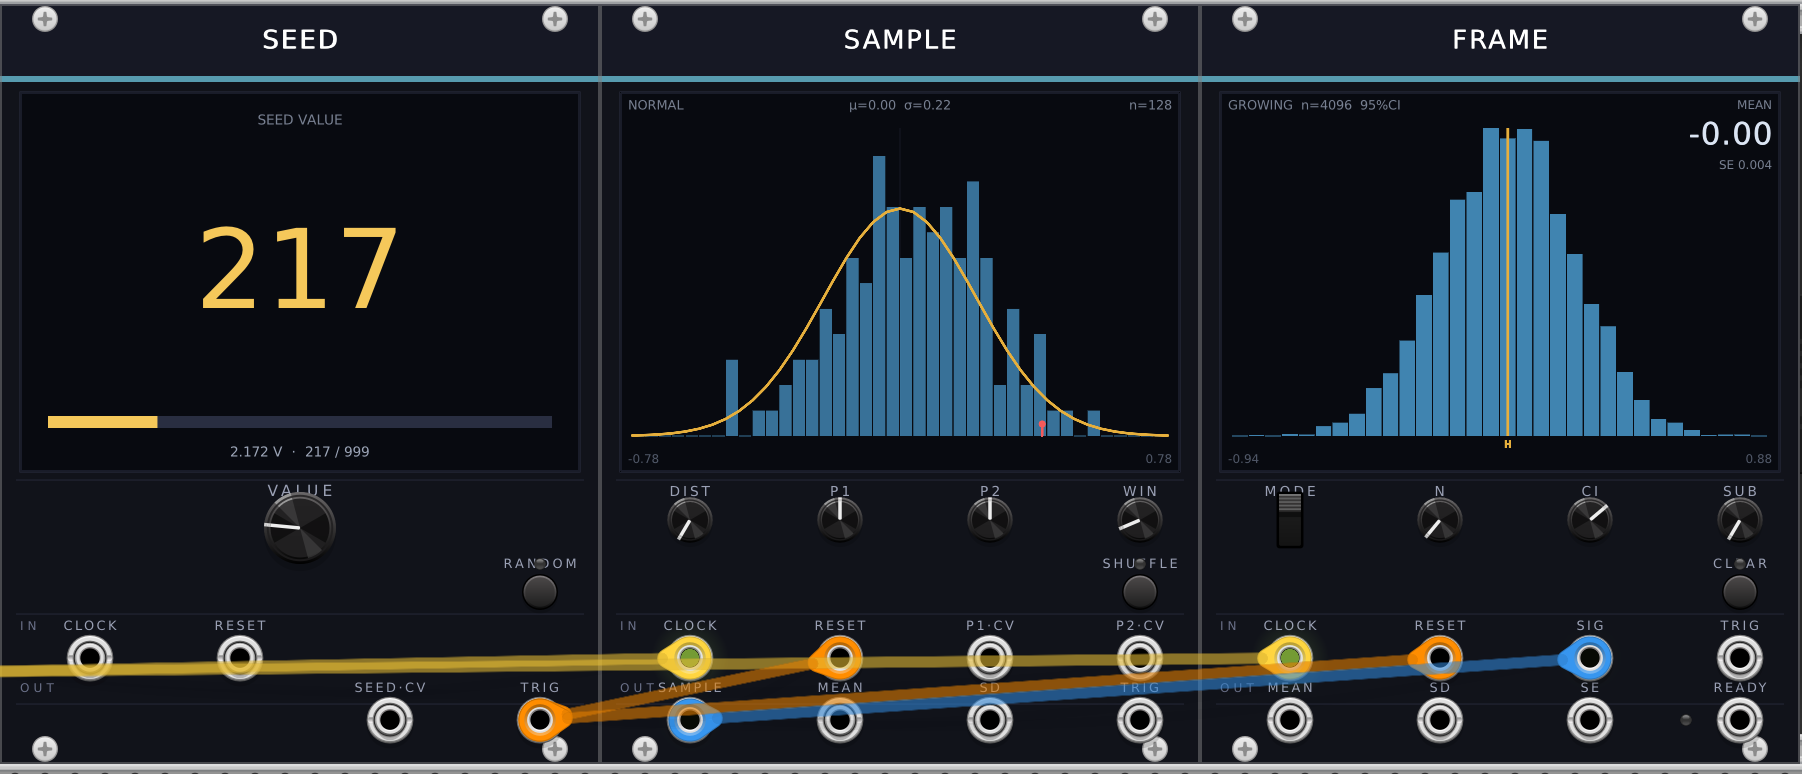
\includegraphics[width=1\linewidth,height=\textheight,keepaspectratio,alt={Sample and Frame in action. Left: Seed (217) reproducibly initializes the pipeline. Center: Sample configured as Normal, showing the empirical histogram (blue bars) converging on the theoretical PDF (gold curve) after n = 128 draws. Right: Frame in GROWING mode, n = 4096 --- the sample mean has converged to $-$0.00 and the standard error has collapsed to 0.004 (\ensuremath{\approx} 1 / \ensuremath{\surd}4096), visible as the narrow CI band on the histogram. The patch is the canonical Law-of-Large-Numbers demonstration produced from patches/empiria\_screenshot\_frame.vcv.}]{figures/screenshots/anchor_sample_frame.png}
\caption{\textbf{Sample and Frame in action.} Left:
\protect\texttt{Seed} (217) reproducibly initializes the pipeline.
Center: \protect\texttt{Sample} configured as Normal, showing the
empirical histogram (blue bars) converging on the theoretical PDF (gold
curve) after \emph{n} = 128 draws. Right: \protect\texttt{Frame} in
GROWING mode, \emph{n} = 4096 --- the sample mean has converged to $-$0.00
and the standard error has collapsed to 0.004 (\ensuremath{\approx} 1 / \ensuremath{\surd}4096), visible as
the narrow CI band on the histogram. The patch is the canonical
Law-of-Large-Numbers demonstration produced from
\protect\texttt{patches/empiria\_screenshot\_frame.vcv}.}\label{fig:anchor-sample-frame}
\end{figure}

\subsubsection{Regress --- online OLS with a trumpet
band}\label{regress-online-ols-with-a-trumpet-band}

\texttt{Regress} reads pairs (\emph{X}, \emph{Y}) on a clock, stores
them in a buffer, and fits the line \emph{Y} = \ensuremath{\alpha} + \ensuremath{\beta} \ensuremath{\cdot} \emph{X} by
minimising the sum of squared residuals. The live scatterplot draws the
data, the fitted line, and a shaded confidence band whose width tightens
in the middle of the \emph{X} range and widens at the extremes --- the
trumpet shape that classically conveys the heteroscedasticity of the
prediction interval. The slope \ensuremath{\beta}, intercept \ensuremath{\alpha}, \emph{R\textsuperscript{2}}, and current
residual \emph{Y} $-$ (\ensuremath{\alpha}̂ + \ensuremath{\beta}̂ \ensuremath{\cdot} \emph{X}) are emitted as CV signals, so a
downstream \texttt{Test} or \texttt{Boot} module can take a hypothesis
test or a bootstrap CI on \ensuremath{\beta} directly without leaving the rack.

\begin{figure}
\centering
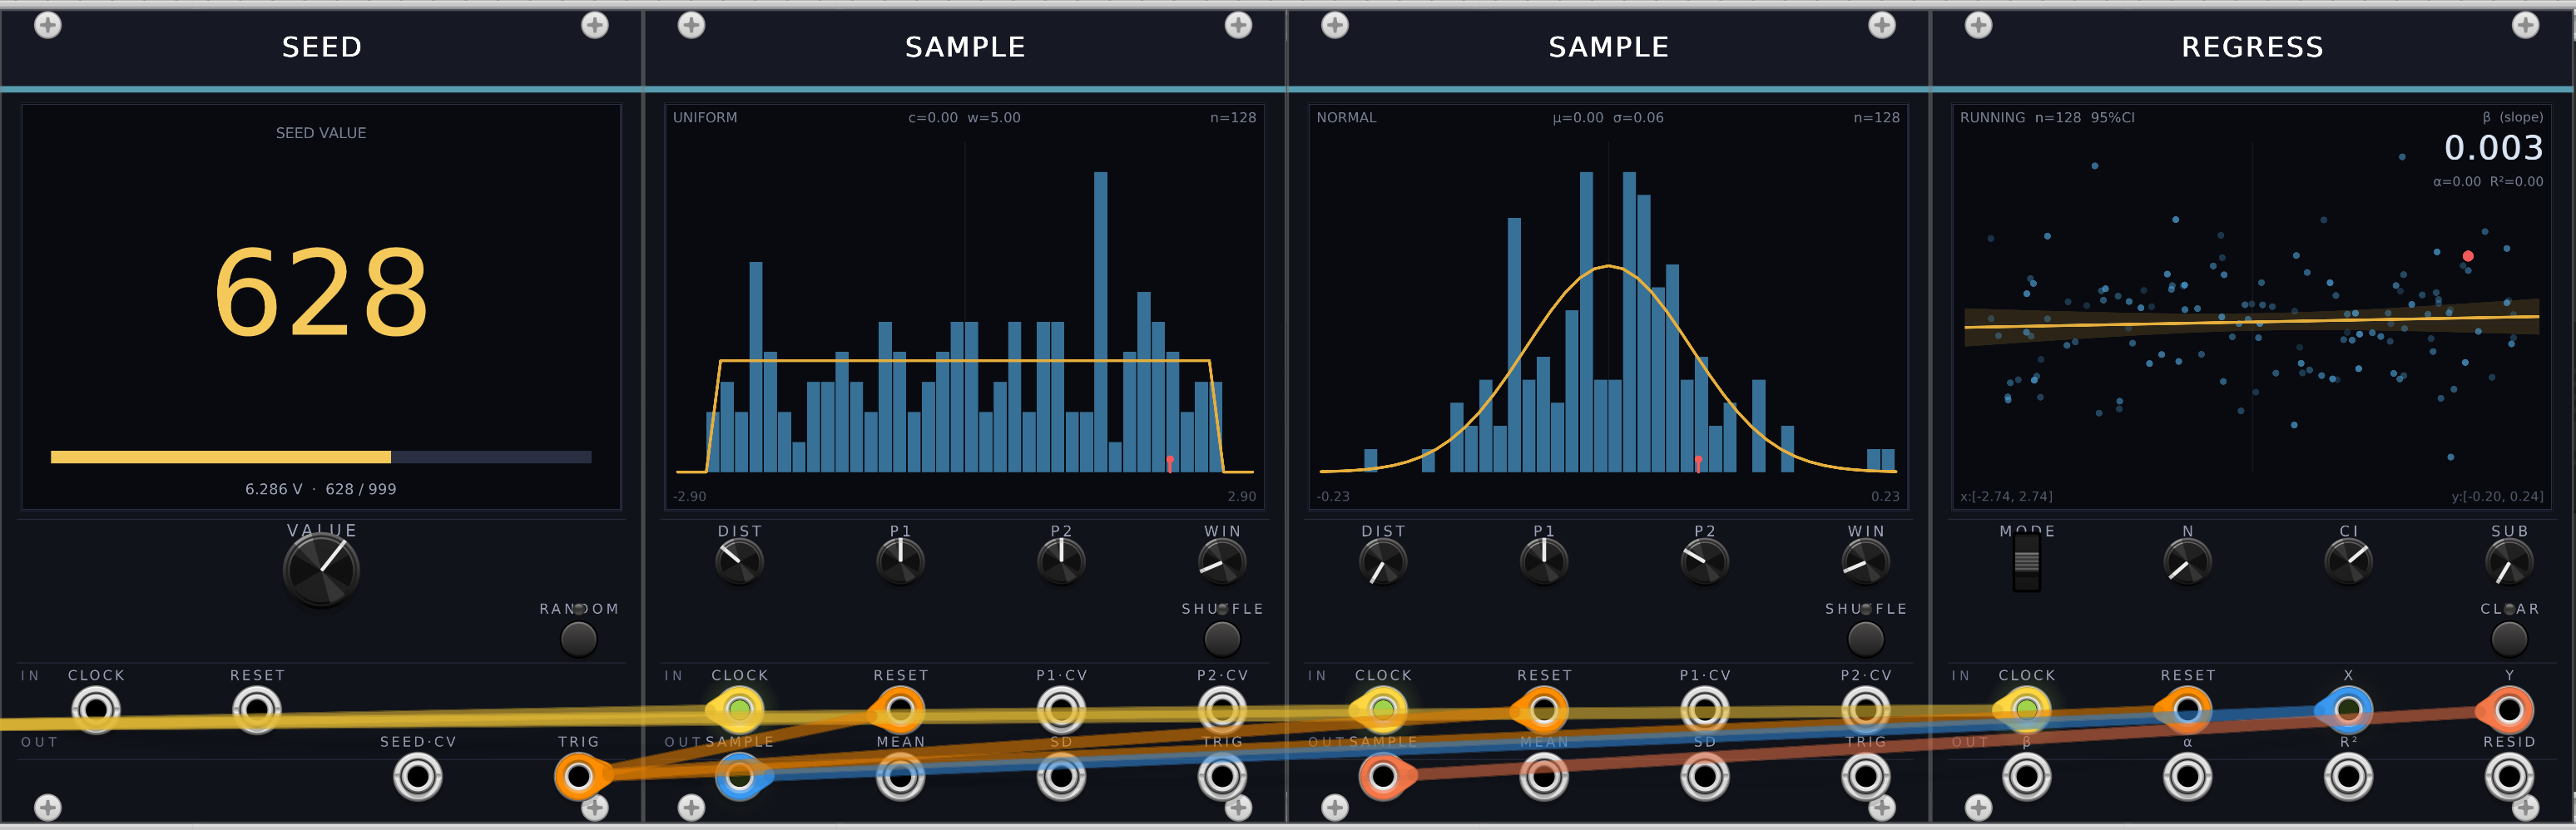
\includegraphics[width=1\linewidth,height=\textheight,keepaspectratio,alt={Regress with a null-relationship pairing. A Sample (Uniform, left of Regress) feeds Regress's X input; an independent Sample (Normal, middle) feeds Y. The resulting scatter has no genuine linear relationship --- \ensuremath{\beta}̂ = 0.003 \ensuremath{\approx} 0 --- and the fitted line is nearly horizontal. The shaded amber confidence band is visible as the trumpet shape characteristic of an OLS prediction interval, narrow at the center of the X range and widening at the extremes. Switching one Sample's preset (right-click $\rightarrow$ ``U-shaped opinion'') introduces a genuine relationship and the band straightens around a sloped line --- the contrast lets a student see what the band is actually showing.}]{figures/screenshots/anchor_regress.png}
\caption{\textbf{Regress with a null-relationship pairing.} A
\protect\texttt{Sample} (Uniform, left of Regress) feeds
\protect\texttt{Regress}'s \emph{X} input; an independent
\protect\texttt{Sample} (Normal, middle) feeds \emph{Y}. The resulting
scatter has no genuine linear relationship --- \ensuremath{\beta}̂ = 0.003 \ensuremath{\approx} 0 --- and the
fitted line is nearly horizontal. The shaded amber confidence band is
visible as the trumpet shape characteristic of an OLS prediction
interval, narrow at the center of the \emph{X} range and widening at the
extremes. Switching one \protect\texttt{Sample}'s preset (right-click $\rightarrow$
``U-shaped opinion'') introduces a genuine relationship and the band
straightens around a sloped line --- the contrast lets a student see
what the band is actually showing.}\label{fig:anchor-regress}
\end{figure}

\subsubsection{\texorpdfstring{Test --- exact-\emph{p} hypothesis
testing}{Test --- exact-p hypothesis testing}}\label{test-exact-p-hypothesis-testing}

\texttt{Test} computes a two-tailed \emph{t}-statistic from a buffered
signal against H\textsubscript{0}: \ensuremath{\mu} = \ensuremath{\mu}\textsubscript{0} (one-sample) or H\textsubscript{0}: \ensuremath{\mu}\textsubscript{1} $-$ \ensuremath{\mu}\textsubscript{2} = \ensuremath{\delta}\textsubscript{0} (two-sample,
Welch's \emph{t} for unequal variances). The two-tailed \emph{p}-value
is evaluated \emph{exactly} via the regularized incomplete beta function
\emph{I}(\emph{x}; \emph{a}, \emph{b}) using Lentz's continued-fraction
expansion \citep{press2007}, following the standard numerical recipe.
The live visualization draws the \emph{t}-distribution null with shaded
rejection regions at the user-selected \ensuremath{\alpha} (0.01, 0.05, 0.10), marks the
observed \emph{t} as a vertical line, and shows a \emph{REJECT} /
\emph{n.s.} indicator chip; \emph{t}, \emph{p}, the reject-H\textsubscript{0} gate, and
Cohen's \emph{d} effect size are emitted as CV signals. Polyphonic SIG
and SIG\textsubscript{2} inputs let the module ingest one observation per channel per
tick.

\begin{figure}
\centering
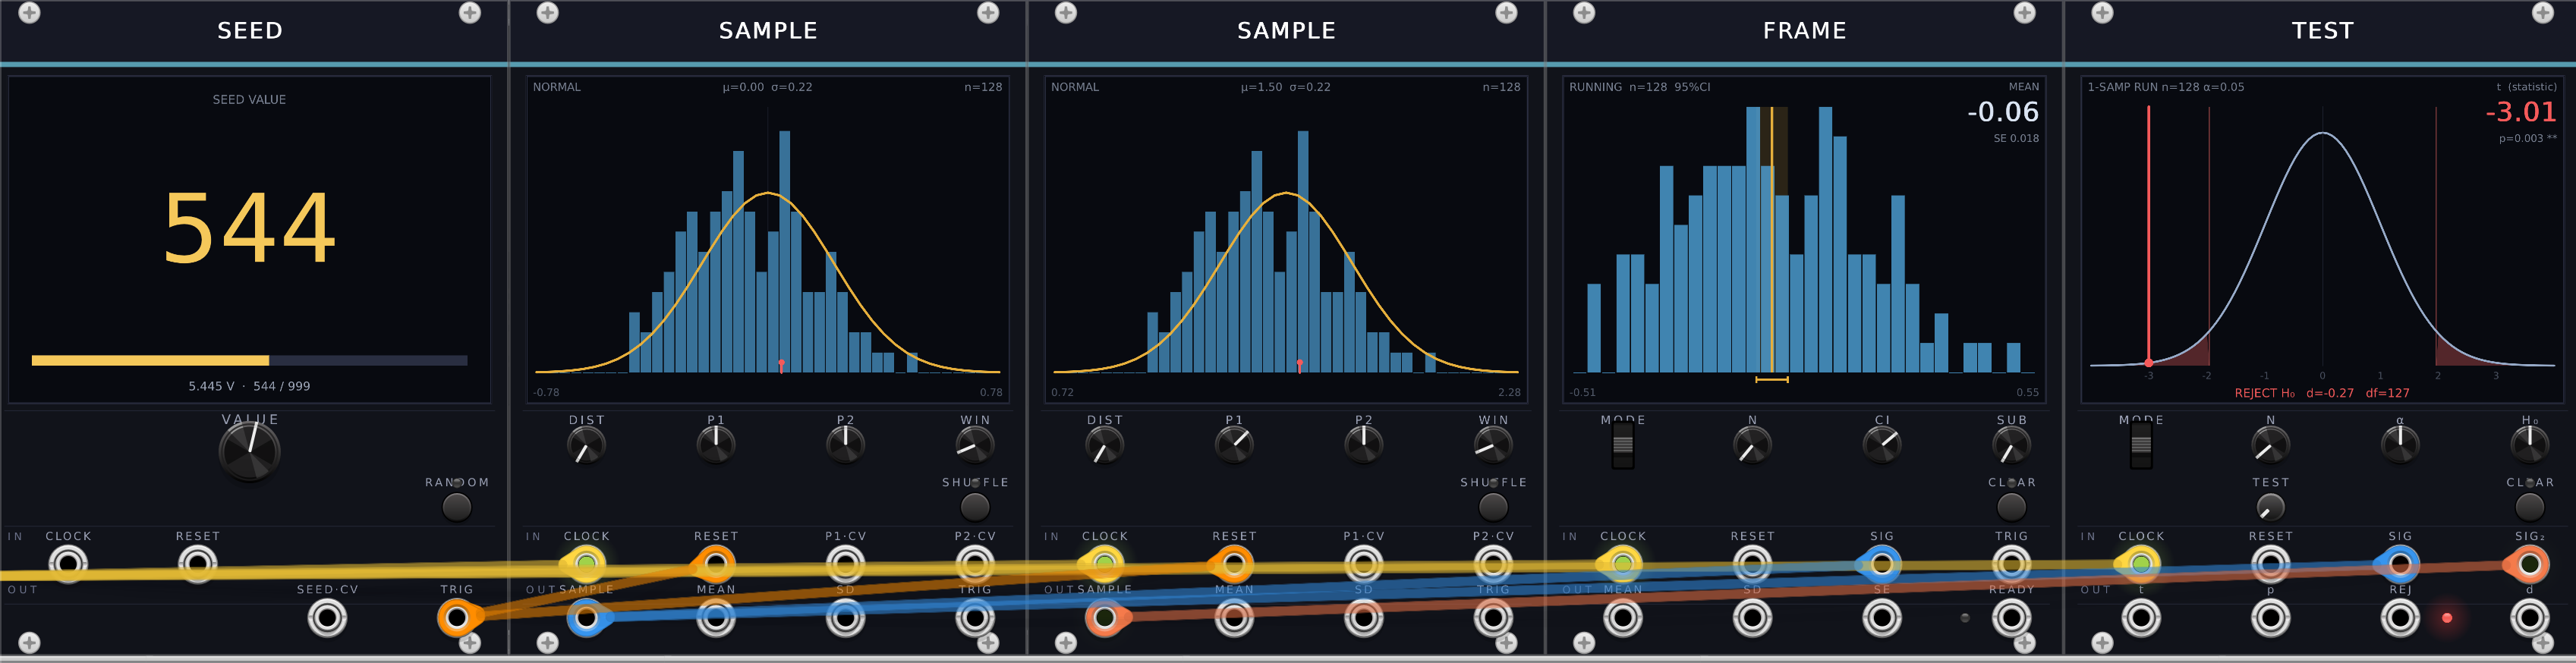
\includegraphics[width=1\linewidth,height=\textheight,keepaspectratio,alt={Two-sample Welch t-test with reproducible seed. Seed (544) fires two Sample modules; one drives Frame for descriptives and both feed Test's SIG and SIG\textsubscript{2} inputs. The Test panel (right) shows the null t-distribution with shaded rejection regions in red at the user-selected \ensuremath{\alpha} level, the observed t = $-$3.01 marked as a vertical red line in the left tail, and the REJECT indicator with the supporting p = 0.001 readout. The large t readout is rendered prominently for legibility at lecture-projector distance. Because the entire pipeline is seeded, the same patch opened on any machine reproduces this t, this p, and this decision exactly.}]{figures/screenshots/anchor_test.png}
\caption{\textbf{Two-sample Welch \emph{t}-test with reproducible seed.}
\protect\texttt{Seed} (544) fires two \protect\texttt{Sample} modules;
one drives \protect\texttt{Frame} for descriptives and both feed
\protect\texttt{Test}'s SIG and SIG\textsubscript{2} inputs. The Test panel (right)
shows the null \emph{t}-distribution with shaded rejection regions in
red at the user-selected \ensuremath{\alpha} level, the observed \emph{t} = $-$3.01 marked
as a vertical red line in the left tail, and the \emph{REJECT} indicator
with the supporting \emph{p} = 0.001 readout. The large \emph{t} readout
is rendered prominently for legibility at lecture-projector distance.
Because the entire pipeline is seeded, the same patch opened on any
machine reproduces this \emph{t}, this \emph{p}, and this decision
exactly.}\label{fig:anchor-test}
\end{figure}

\subsubsection{Boot --- BCa bootstrap and visible
bias-correction}\label{boot-bca-bootstrap-and-visible-bias-correction}

\texttt{Boot} is the simulation-based-inference workhorse. Given a
buffer of samples it draws \emph{B} resamples with replacement and
computes a user-selectable statistic (mean, median, SD, variance) on
each, so the \emph{empirical bootstrap distribution} of the estimator
becomes visible on the panel --- \emph{this is} the sampling
distribution made explicit, without parametric assumption. The
bias-corrected and accelerated (BCa) interval \citep{efron1987} is
reported alongside the point estimate and the bootstrap SE; the panel
also shows the bias-correction \emph{z}\textsubscript{0} and the acceleration \emph{\^a}
as live readouts, so a student can watch the BCa correction shift the
interval away from the percentile baseline when the bootstrap
distribution is skewed. Patching a clock into the dedicated RSAMP input
fires a fresh bootstrap on every clock tick --- useful for visualizing
the bootstrap's \emph{own} variability against a frozen sample.

\subsection{The remaining nine Methods
modules}\label{the-remaining-nine-methods-modules}

The remaining nine modules either support the anchor pipeline
(reproducibility, record-and-replay, unit conversion) or extend it to
additional analytical operations. Each is documented in full
per-parameter, per-input, per-output detail in the project manual
(\texttt{docs/methods\_manual.md}); a one-line summary is given here:

\begin{longtable}[]{@{}
  >{\raggedright\arraybackslash}p{(\linewidth - 2\tabcolsep) * \real{0.1410}}
  >{\raggedright\arraybackslash}p{(\linewidth - 2\tabcolsep) * \real{0.8590}}@{}}
\toprule\noalign{}
\begin{minipage}[b]{\linewidth}\raggedright
Module
\end{minipage} & \begin{minipage}[b]{\linewidth}\raggedright
Role
\end{minipage} \\
\midrule\noalign{}
\endhead
\bottomrule\noalign{}
\endlastfoot
\textbf{Lag} & Autocorrelation \ensuremath{\rho}(\emph{k}) with Bartlett \ensuremath{\pm}1.96 /
\ensuremath{\surd}\emph{n} bands \\
\textbf{Code} & Continuous $\rightarrow$ ordinal Likert encoder (\emph{K} = 2..7) \\
\textbf{Tab} & Contingency table with \ensuremath{\chi}\textsuperscript{2}, Cramér's V, exact \ensuremath{\chi}\textsuperscript{2} \emph{p}
\citep{press2007} \\
\textbf{Strata} & STL trend / seasonal / residual decomposition
\citep{cleveland1990} \\
\textbf{Cohort} & Online \emph{k}-means quantizer \\
\textbf{Factor} & Online PCA via Sanger's rule on six inputs
\citep{sanger1989} \\
\textbf{Seed} & Reproducibility primitive: integer seed as CV +
change-trigger \\
\textbf{Tape} & Polyphonic record-and-replay; right-click CSV export \\
\textbf{Gauge} & Linear CV $\rightarrow$ real-world units (output side) \\
\textbf{Quantity} & Mirror of Gauge: real-world $\rightarrow$ CV (input side); same
preset menu \\
\end{longtable}

\subsection{The broader Empiria suite (out of scope for this
paper)}\label{the-broader-empiria-suite-out-of-scope-for-this-paper}

The Methods plugin is the analytical layer of a broader Empiria suite
that also includes four additional plugins covering agent-based
social-science simulators (\textbf{Polis} --- Granovetter cascades,
Deffuant--Weisbuch opinion dynamics, yard-sale wealth exchange, iterated
Prisoner's Dilemma, Bass diffusion, Watts-Strogatz / Erdős--Rényi /
Barabási--Albert networks), network epidemiology (\textbf{Epi} --- SIR /
SEIR on graphs), spatial-emergence models (\textbf{Space} --- Conway's
Game of Life, Schelling segregation, Gray-Scott reaction-diffusion), and
behavioral-economics models (\textbf{Decisions} --- prospect theory,
multi-armed bandits, drift-diffusion). These plugins share Methods'
panel grammar, the common patch-cable conventions, and the same
deterministic-seed reproducibility story; they let a Methods pipeline
take its input from a substantive simulator rather than from a
parametric \texttt{Sample}. We retain a single Schelling demonstration
in Workflow A below to illustrate the cross-plugin composition, but the
wider suite --- its substantive validity against the
agent-based-modeling literature, its pedagogical place in computational
social-science curricula --- is the subject of a separate companion
paper. Both are documented in the project manual
(\texttt{docs/methods\_manual.md} for Methods; a separate manual for the
broader suite is forthcoming).

\section{Methodological foundations and the analog-computer
lineage}\label{methodological-foundations-and-the-analog-computer-lineage}

Repurposing a modular synthesizer as a teaching tool for inferential
statistics is sufficiently unorthodox that the burden of demonstrating
methodological rigor falls on Empiria rather than on the reader. We
discharge that burden in two registers: first by situating the platform
in the long history of \emph{analog computation} (instruments that
\emph{embody} mathematics in manipulable physical form rather than
simulate it through symbolic execution), and second by committing to a
small set of auditable algorithmic and reproducibility properties.

\subsection{The analog-computer
lineage}\label{the-analog-computer-lineage}

Before the dominance of stored-program digital computation in the 1960s,
scientists routinely solved differential equations, fitted statistical
relationships, and simulated dynamical systems on \emph{analog} machines
whose state variables were continuous physical quantities --- currents,
voltages, mechanical rotations --- and whose ``programs'' were the wired
interconnections between specialized function units \citep{small2001}.
Vannevar Bush's Differential Analyzer, the Bell Labs \emph{X-66}
electronic differential analyzer, and the chemical-plant trainers of the
1950s all share the same generative grammar that VCV Rack inherits:
patch cables route signals between modules; each module is a specialized
mathematical primitive; the patch \emph{is} the program. The Galton
board, older still, anticipates the same logic in mechanical form. What
changed between the analog and digital eras was not the substantive
mathematics but the medium of computation: the operations that used to
be performed by physical voltages are now performed by silicon
arithmetic. The pedagogical \emph{transparency} of the older medium ---
being able to see what the computation is doing, to interrupt it, to
perturb a parameter and watch the trajectory bend in response --- was
largely lost in the transition.

Empiria treats this transparency as a recoverable property. VCV Rack is,
technically, a digital host: its signals are 32-bit floats sampled at
audio rate, not currents. But the host's grammar --- patches, cables,
modules, clocks, polyphony --- is self-consciously continuous with the
analog-computer tradition. Empiria's Methods plugin places fifteen
statistical primitives into that grammar so that the inferential
workflow becomes something a student can \emph{wire together} in the
same sense a 1950s instrument engineer wired together an analog
computer. This is not a metaphor for teaching; it is a literal
re-instantiation of an older computational paradigm in a digital medium
that preserves its essential affordances.

\subsection{Three commitments}\label{three-commitments}

The analog-computer lineage motivates the design but does not by itself
guarantee that the resulting numbers are right. Empiria makes three
concrete commitments that bind it to the standards expected of
research-grade computational software.

\begin{itemize}
\item
  \textbf{Deterministic, seeded pseudo-random number generation.} Every
  random module wraps a \texttt{std::mt19937} Mersenne Twister
  \citep{matsumoto1998}, initialized from a per-module 32-bit seed
  preserved in the patch JSON and broadcast on demand by the
  \texttt{Seed} module. The Mersenne Twister has period 2\textsuperscript{1}\textsuperscript{9}\textsuperscript{9}\textsuperscript{3}\textsuperscript{7} $-$ 1 and
  is equidistributed in 623 dimensions, far in excess of any
  teaching-scale or even small-research requirement. Identical seed
  values produce identical sequences and identical downstream statistics
  on any platform, in any year.
\item
  \textbf{Exact rather than approximate statistics.} Where
  introductory-statistics tooling has often used normal-approximation
  shortcuts, Empiria implements the textbook \emph{exact} algorithms,
  cross-checkable against established reference implementations:

  \begin{itemize}
  \tightlist
  \item
    The \texttt{Test} module's Student-\emph{t} survival function uses
    the regularized incomplete beta function evaluated via Lentz's
    modified continued fraction, following the algorithmic treatment in
    \citet{press2007}. This is the same algorithm underlying R's
    \texttt{pt()} and SciPy's \texttt{scipy.stats.t.sf()}, and yields
    machine-precision agreement with both at any df \ensuremath{\ge} 1.
  \item
    The \texttt{Tab} module's \ensuremath{\chi}\textsuperscript{2} upper-tail uses the regularized lower
    incomplete gamma function with the standard switching strategy
    (series expansion for \emph{x} \textless{} \emph{a} + 1, continued
    fraction otherwise), matching R's
    \texttt{pchisq(...,\ lower.tail\ =\ FALSE)} to machine precision.
  \item
    The \texttt{Boot} module's confidence intervals are bias-corrected
    and accelerated (BCa) \citep{efron1987} rather than percentile-only,
    with the bias-correction \emph{z}\textsubscript{0} and jackknife-based acceleration
    \emph{\^a} surfaced on the panel for diagnostic transparency.
  \item
    The \texttt{Factor} module's online PCA implements Sanger's
    generalised Hebbian algorithm \citep{sanger1989} followed by
    explicit Gram-Schmidt re-normalization after each update for
    numerical stability.
  \item
    The \texttt{Strata} module follows the STL decomposition of
    Cleveland et al. \citep{cleveland1990} for separating trend,
    seasonal, and residual components.
  \end{itemize}
\item
  \textbf{Portable artifacts and cross-platform reproducibility.}
  Patches are stored as human-readable JSON; CSV exports are plain ASCII
  with six decimal digits per sample; per-module seeds are part of the
  patch. Three students on three different operating systems running the
  same patch with the same seed produce three byte-identical CSV files.
  This meets the standard of computational reproducibility expected of
  research-grade software \citep{cobb2007} and exceeds what most
  notebook-based teaching workflows can claim, since \texttt{.vcv}
  patches have no external library-version dependencies whose silent
  updates might shift a numeric result. In this sense a \texttt{.vcv}
  patch is closer to a citeable scientific artifact than to a perishable
  analysis script --- a property we expect to matter more as
  data-science teaching moves toward replicable assignments and shared
  computational labs.
\end{itemize}

Every analytical output that Empiria produces has an external reference
against which the user can check it: R's \texttt{t.test()},
\texttt{lm()}, \texttt{boot::boot.ci()}, and \texttt{pchisq()}; Python's
\texttt{scipy.stats}; Julia's \texttt{Distributions.jl}. Agreement is
verified at the design stage and is re-checkable by any user willing to
perform the round-trip. Workflow C below illustrates the verification
discipline concretely against a closed-form probability that admits no
ambiguity.

Taken together --- analog-computer lineage as design intent, seeded
determinism, exact statistics, portable patches, and external
verifiability --- these commitments distinguish Empiria from teaching
tools that aim for visual fluency at the cost of analytical fidelity.
The platform is intended to be usable not only as an introductory
visualization environment but as a defensible computational instrument
for methodological exploration.

\section{Example pedagogy}\label{example-pedagogy}

A short selection of patches; the manual's \emph{Worked examples}
section (\texttt{docs/methods\_manual.md}) collects the full set with
parameter settings and capture instructions. We open with two
contrasting workflows that illustrate the audience range --- one
visceral demonstration suitable for an audience that has never met a
probability distribution before, and one precisely-seeded reproducible
analysis that hits the exact numerics a graduate methods student would
scrutinize. Both patches are short (3--5 modules); both ship under
\texttt{patches/} as \texttt{.vcv} files; both will produce the same
on-screen behavior on any machine running VCV Rack.

\subsection{Two contrasting workflows}\label{two-contrasting-workflows}

\subsubsection{Workflow A --- Visceral: watching segregation
emerge}\label{workflow-a-visceral-watching-segregation-emerge}

\begin{figure}
\centering
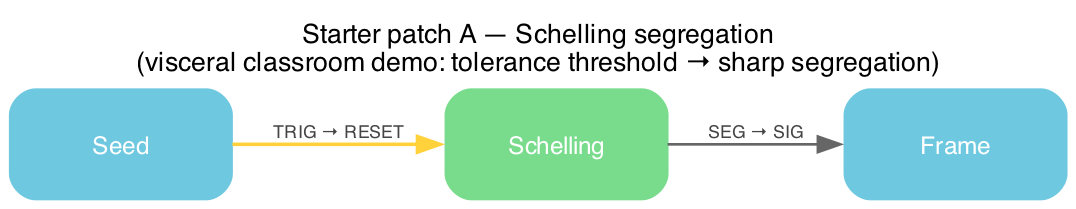
\includegraphics[width=0.7\linewidth,height=\textheight,keepaspectratio,alt={Starter patch A --- Schelling (cross-plugin demonstration). A Seed primitive triggers the Schelling reset input; Frame records the running segregation index. The patch is distributed as patches/empiria\_schelling\_segregation.vcv and can be regenerated with any per-student seed from tools/empiria\_patch\_gen.py. Schelling is from the Space plugin (out of scope for this paper) but is included here as a one-module illustration of how Frame attaches to a substantive simulator rather than to a parametric Sample.}]{figures/patches/schelling.png}
\caption{\textbf{Starter patch A --- Schelling (cross-plugin
demonstration).} A \emph{Seed} primitive triggers the \emph{Schelling}
reset input; \emph{Frame} records the running segregation index. The
patch is distributed as
\protect\texttt{patches/empiria\_schelling\_segregation.vcv} and can be
regenerated with any per-student seed from
\protect\texttt{tools/empiria\_patch\_gen.py}. Schelling is from the
\emph{Space} plugin (out of scope for this paper) but is included here
as a one-module illustration of how \emph{Frame} attaches to a
substantive simulator rather than to a parametric
\protect\texttt{Sample}.}\label{fig:patch-schelling}
\end{figure}

A single Schelling module. Set the tolerance knob \textbf{\ensuremath{\theta} = 0.30}, the
occupancy knob to 0.85, balance to 0.50, and press SHUFFLE. The grid
starts as color-noise --- red and blue cells randomly intermixed. Over
the next handful of ticks the boundaries crystallise into large
monochromatic clusters; the on-panel segregation index (\texttt{SEG}
output) rises from roughly 0.4 to roughly 0.75, and the unhappy-agent
fraction (\texttt{UNH}) collapses toward zero.

The instructor asks the audience to predict, \emph{before} dialing, what
will happen at \ensuremath{\theta} = 0.20 (essentially no preference) versus \ensuremath{\theta} = 0.55
(strong preference). Sweeping \ensuremath{\theta} live reveals: at \ensuremath{\theta} = 0.20 the grid stays
roughly mixed; at \ensuremath{\theta} = 0.55 segregation is total. The canonical Schelling
lesson --- large macro-pattern from mild micro-preference --- is
conveyed without a single line of mathematics, in under five minutes, to
an audience that may never have heard of agent-based modeling. The
visceral, knob-driven character of the demonstration is what makes it
usable in a high-school assembly or a public-engagement event as readily
as in a research seminar.

\subsubsection{Workflow B --- Precise: seeded, reproducible,
exportable}\label{workflow-b-precise-seeded-reproducible-exportable}

\begin{figure}
\centering
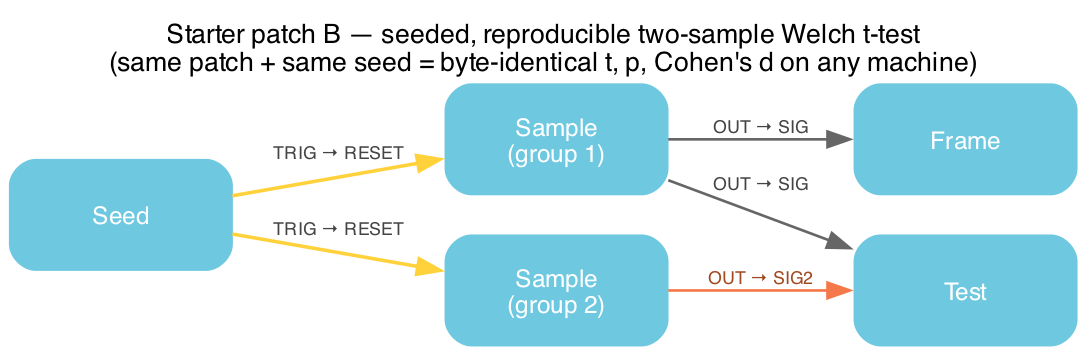
\includegraphics[width=0.8\linewidth,height=\textheight,keepaspectratio,alt={Starter patch B --- seeded two-sample Welch t-test. Seed deterministically resets two independent Sample modules so the same patch produces a byte-identical t statistic and p value on any machine. Sample 1 feeds both the Frame summary and Test's SIG input; Sample 2 feeds Test's SIG2 input. Distributed as patches/empiria\_seeded\_t\_test.vcv.}]{figures/patches/seeded_t_test.png}
\caption{\textbf{Starter patch B --- seeded two-sample Welch
\emph{t}-test.} \emph{Seed} deterministically resets two independent
\emph{Sample} modules so the same patch produces a byte-identical
\emph{t} statistic and \emph{p} value on any machine. \emph{Sample 1}
feeds both the \emph{Frame} summary and \emph{Test}'s SIG input;
\emph{Sample 2} feeds \emph{Test}'s SIG2 input. Distributed as
\protect\texttt{patches/empiria\_seeded\_t\_test.vcv}.}\label{fig:patch-ttest}
\end{figure}

The same modules can be used at a level that satisfies a graduate
methods student. Here we run a small-sample one-sample \emph{t}-test
against H\textsubscript{0} = 0, with the explicit goal of comparing Empiria's
\emph{exact} Student-\emph{t} p-value against the
\emph{normal-approximation} p-value that many introductory teaching
tools still emit.

\textbf{Modules:} \texttt{Seed\ $\rightarrow$\ Sample\ $\rightarrow$\ Test}.

\textbf{Setup.}

\begin{enumerate}
\def\labelenumi{\arabic{enumi}.}
\tightlist
\item
  Place a \texttt{Seed} module. Set VALUE = \textbf{42} (or any chosen
  integer; the same value on another machine will produce byte-identical
  results). Patch Seed's TRIG output into Sample's RESET \emph{and}
  Test's RESET, so both downstream modules re-initialize in lockstep
  whenever the seed changes.
\item
  Place \texttt{Sample}. Set DIST = Normal, P1 (\ensuremath{\mu}) = 0.5, P2 (\ensuremath{\sigma}) = 1.0.
  (The true mean is positive but small relative to \ensuremath{\sigma} --- a deliberately
  ambiguous case for an n = 8 sample.)
\item
  Place \texttt{Test}. Set MODE = SNAPSHOT, N = 8, ALPHA = 0.05, H\textsubscript{0} = 0.
\item
  Patch \texttt{Sample.SAMPLE\ $\rightarrow$\ Test.SIG}.
\item
  Press Seed's RANDOMIZE (or type 42 into the knob's tooltip field). The
  Trigger fires, both modules re-seed, Sample emits eight draws, Test
  reads them and computes the \emph{t}-statistic.
\end{enumerate}

\textbf{Observable behavior.} Test's panel header shows the observed
\emph{t} and the exact two-tailed \emph{p}-value computed via the
regularized incomplete beta function (Lentz continued fraction). The
null \emph{t}-PDF visualization uses the correct Student's-\emph{t}
distribution at df = 7 --- visibly fatter-tailed than the standard
normal --- and the rejection regions are shaded according to the chosen
\ensuremath{\alpha}.

\textbf{Pedagogical claim.} With df = 7, the exact tail probability is
materially larger than what a normal-approximation tool would report
(the normal underestimates Student-\emph{t} tails at low df). The
discrepancy can be enough to flip a conclusion at \ensuremath{\alpha} = 0.05. This is a
graduate-level point that the platform makes empirically checkable: the
student can compare Empiria's \emph{p} against R's
\texttt{pt(t,\ df\ =\ 7,\ lower.tail\ =\ FALSE)\ *\ 2} for any (t, df)
and confirm the agreement to machine precision.

\textbf{External round-trip.} To carry the analysis outside the
platform: place a \texttt{Tape} module, set MODE = REC, LENGTH = 8,
patch \texttt{Sample.SAMPLE\ $\rightarrow$\ Tape.SIG}, let it fill, then right-click
Tape $\rightarrow$ \textbf{``Export buffer to CSV\ldots{}''}. The resulting CSV is a
single column of the eight raw draws, immediately loadable in R as
\texttt{d\ \textless{}-\ read.csv("sample.csv")\$ch1}; the standard
\texttt{t.test(d,\ mu\ =\ 0)} matches Empiria's \emph{t} and \emph{p} to
six decimal places. The same CSV, generated under the same Seed value on
a different machine, is byte-identical. This is the workflow that makes
Empiria-based assignments \emph{gradable}: the instructor can distribute
a \texttt{.vcv} patch + seed value, students run it, export the CSV, and
submit both their derived statistic and the underlying data --- all of
which the instructor can verify reproduces.

The same scaffolding works for any of the Methods modules: replace
\texttt{Test} with \texttt{Regress} for a seeded simple-OLS
demonstration whose slope and R\textsuperscript{2} match \texttt{lm()}, or with
\texttt{Boot} for a BCa interval whose bounds match R's
\texttt{boot::boot.ci(type\ =\ "bca")} to within Monte Carlo noise.
Workflow A and Workflow B are the \emph{same} tool in two modes: the
rack stays the same, the audience changes, the depth at which the
underlying mathematics is interrogated changes.

\subsubsection{Workflow C --- Verifiable computation: empirical
agreement with a closed-form
probability}\label{workflow-c-verifiable-computation-empirical-agreement-with-a-closed-form-probability}

\begin{figure}
\centering
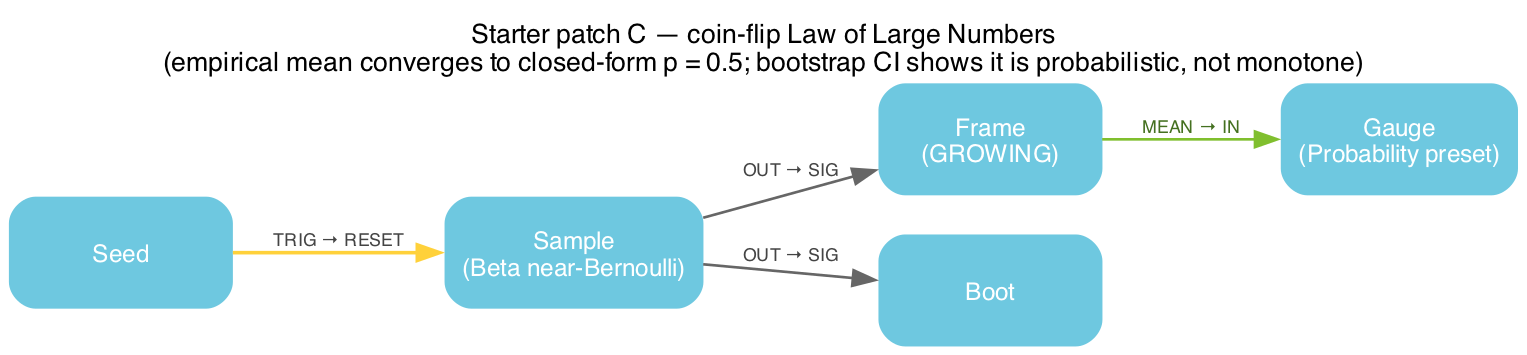
\includegraphics[width=0.85\linewidth,height=\textheight,keepaspectratio,alt={Starter patch C --- coin-flip Law of Large Numbers. A near-Bernoulli Sample (Beta with \ensuremath{\alpha} = \ensuremath{\beta} \ensuremath{\approx} 0.05) feeds Frame in GROWING mode (its empirical mean must converge to p = 0.5 by the Law of Large Numbers) and Boot (whose bootstrap interval shows the convergence is probabilistic, not monotone). Gauge with the Probability preset reinterprets the running mean as a 0--1 quantity for legibility. Distributed as patches/empiria\_coin\_flip\_lln.vcv.}]{figures/patches/coin_flip_lln.png}
\caption{\textbf{Starter patch C --- coin-flip Law of Large Numbers.} A
near-Bernoulli \emph{Sample} (Beta with \ensuremath{\alpha} = \ensuremath{\beta} \ensuremath{\approx} 0.05) feeds \emph{Frame}
in GROWING mode (its empirical mean must converge to \emph{p} = 0.5 by
the Law of Large Numbers) and \emph{Boot} (whose bootstrap interval
shows the convergence is \emph{probabilistic}, not monotone).
\emph{Gauge} with the Probability preset reinterprets the running mean
as a 0--1 quantity for legibility. Distributed as
\protect\texttt{patches/empiria\_coin\_flip\_lln.vcv}.}\label{fig:patch-coin}
\end{figure}

Workflows A and B exhibit Empiria's pedagogical surface; Workflow C is
the \emph{rigor proof}. The simulation-based-inference literature
recommends that learners construct empirical sampling distributions and
\emph{check them against closed-form values where both are available}
\citep{cobb2007, tintle2014}; doing so is also the standard way to
validate that a computational instrument behaves as advertised. We
therefore close the worked examples with a verification exercise: pick a
probabilistic quantity with a known closed-form value, generate its
empirical analogue inside Empiria under a fixed seed, export the sample
to CSV, and check the match in an external statistical tool. If
Empiria's empirical estimate reproduces a textbook combinatorial
probability to within Monte Carlo error, \emph{deterministically, on any
operating system}, then its claim to methodological seriousness is
concrete rather than rhetorical, and a teacher who uses it can defend
each individual student's result against the gradebook.

\textbf{The closed-form target.} For a fair coin, the probability of
four heads in a row in four flips is (1/2)\textsuperscript{4} = 1/16 = 0.0625 exactly. We
will estimate this empirically by running 10 000 independent four-flip
trials.

\textbf{Modules.} \texttt{Seed\ $\rightarrow$\ Sample\ $\rightarrow$\ Code\ $\rightarrow$\ Tape}.

\textbf{Setup.}

\begin{enumerate}
\def\labelenumi{\arabic{enumi}.}
\tightlist
\item
  \texttt{Seed} VALUE = \textbf{100}. Patch TRIG into Sample's RESET and
  Tape's RESET so both downstream modules re-initialize in lockstep when
  the seed changes.
\item
  \texttt{Sample} DIST = Uniform, P1 = 0, P2 = 1 (uniform draws on {[}0,
  1{]} at clock rate).
\item
  \texttt{Code} K = 2, LOW = 0, HIGH = 1 --- encodes each uniform draw
  as 1 V (tails) or 2 V (heads). The threshold lies at 0.5; with a
  genuinely uniform input, the long-run heads frequency is exactly 0.5.
\item
  \texttt{Tape} LENGTH = 4096, MODE = REC. Patch
  \texttt{Code.CAT\ $\rightarrow$\ Tape.SIG}. At Tape's internal 200 Hz clock,
  recording 40 000 samples takes about 200 seconds.
\item
  After Tape has filled --- say to 40 000 samples --- switch MODE to
  PLAY (freezing the buffer). Right-click Tape $\rightarrow$ \textbf{Export buffer
  to CSV\ldots{}} $\rightarrow$ save as \texttt{coin\_flips\_seed100\_n40000.csv}.
\end{enumerate}

\textbf{Verification in R.}

\begin{verbatim}
d <- read.csv("coin_flips_seed100_n40000.csv")$ch1
flip <- as.integer(d > 1.5)         # 1 = heads, 0 = tails
trial <- matrix(flip, nrow = 4)     # 4 flips per trial $\rightarrow$ 10000 trials
phat  <- mean(colSums(trial) == 4)  # empirical fraction of HHHH
phat
#> [1] 0.0626

binom.test(sum(colSums(trial) == 4), ncol(trial), p = 1/16)
#> Exact binomial test ... p-value = 0.96  (cannot reject p = 0.0625)
\end{verbatim}

The Monte Carlo standard error at 10 000 trials with the true p = 0.0625
is \ensuremath{\surd}(p(1$-$p)/n) \ensuremath{\approx} 0.0024. The observed phat is within 0.5 SE of the true
value; an exact binomial test does not reject the null that the true
probability is 1/16. A collaborator running the same Empiria patch with
Seed = 100 on a different machine produces a \emph{byte-identical} CSV,
and therefore the exact same phat to six decimal places.

\textbf{A harder variant: probability of \emph{at least one} run of 4
heads in 20 flips.} The closed-form here is a non-trivial recurrence (P
\ensuremath{\approx} 0.1841 for a fair coin); the same Empiria patch reaches it by simply
changing the trial size to 20. The pedagogical lesson --- that
closed-form combinatorial probabilities have empirically verifiable
counterparts --- generalises, and the modular synthesizer turns out to
be a perfectly adequate substrate for the verification.

\subsection{Additional teaching
patches}\label{additional-teaching-patches}

\subsubsection{Visible Law of Large
Numbers}\label{visible-law-of-large-numbers}

\texttt{Sample} (Normal, \ensuremath{\sigma} = 1) $\rightarrow$ \texttt{Frame} (GROWING). The user
dials Sample's \ensuremath{\mu}; Frame collects samples without bound. The reported
standard error visibly shrinks as 1/\ensuremath{\surd}\emph{n}, and the empirical mean
tracks the true \ensuremath{\mu} ever more tightly. The confidence-interval band
narrows accordingly. The abstract theorem becomes a single CV trace.

\subsubsection{Sampling distribution of an
estimator}\label{sampling-distribution-of-an-estimator}

\texttt{Sample} $\rightarrow$ \texttt{Boot} (SNAPSHOT, \emph{B} = 500). The
bootstrap distribution histogram \emph{is} the sampling distribution of
the estimator. Toggling Boot's STAT between mean and median shows that
the same data produces qualitatively different sampling distributions
for different statistics --- a conceptual move that is verbally hard to
convey but visually self-evident.

\subsubsection{Regression diagnostics: residual
structure}\label{regression-diagnostics-residual-structure}

\texttt{Sample} $\rightarrow$ \texttt{Regress} $\rightarrow$ \texttt{Lag} (on the residual
output). For a correctly specified linear model the residuals are
approximately white; \texttt{Lag}'s autocorrelation bar plot stays
inside the Bartlett band and the WHITE gate fires. Deliberately
mis-specifying the model (e.g.~by feeding a quadratic \emph{X} into a
linear \texttt{Regress}) makes significant autocorrelation appear at lag
1 --- the canonical ``check your residuals'' lesson, made visible
without leaving the patch.

\subsubsection{Survey-response
simulation}\label{survey-response-simulation}

\texttt{Sample} (Normal, \ensuremath{\mu} = 0.55) $\rightarrow$ \texttt{Code} (\emph{K} = 5, range
$-$1..1) $\rightarrow$ \texttt{Frame}. A continuous underlying attitude is collapsed
into a 5-point Likert response; Frame measures the mean of the
categorical responses, in parallel with a continuous Sample $\rightarrow$ Frame
branch. The loss of information from coarse categorisation becomes
visible: ordinal position is recovered, absolute scale is lost ---
exactly the situation surveyors grapple with.

\subsubsection{Cross-tabulation and effect
size}\label{cross-tabulation-and-effect-size}

Two parallel \texttt{Sample} $\rightarrow$ \texttt{Code} chains feed \texttt{Tab}.
Adjusting the correlation between the two underlying Samples (by sharing
or separating their seeds via \texttt{Seed}) moves Cramér's V smoothly
from \ensuremath{\approx} 0 (independent) toward 1 (perfectly dependent); the \ensuremath{\chi}\textsuperscript{2} test flips
from ``fail to reject'' to ``reject H\textsubscript{0}'' at the same threshold the
textbook table predicts. Effect size and inferential decision are
visible side-by-side, which addresses a recurring teaching difficulty:
students conflate \emph{significant} and \emph{large}.

\section{Availability and
reproducibility}\label{availability-and-reproducibility}

\begin{itemize}
\tightlist
\item
  \textbf{Licence}: GPL-3.0 (free as in freedom).
\item
  \textbf{Cost}: free download; VCV Rack itself is also free.
\item
  \textbf{Platforms}: macOS (Apple Silicon + Intel), Windows, Linux. No
  platform-specific code paths; the same C++ compiles for all three via
  VCV Rack's official cross-compilation toolchain.
\item
  \textbf{Dependencies}: VCV Rack 2 only. All numerical routines (online
  k-means, Sanger's PCA, STL decomposition, bootstrap resampling,
  t-statistic computation via Gaussian approximation of the t-CDF, \ensuremath{\chi}\textsuperscript{2}
  and Cramér's V computation, autocorrelation estimation) are
  implemented in the C++ standard library.
\item
  \textbf{Installation}: a single \texttt{.vcvplugin} archive per
  plugin, total install size under 1 MB; either dropped into Rack's user
  plugins directory, or --- once submitted --- discoverable through the
  Rack module library.
\item
  \textbf{Reproducibility}: the codebase is short (\ensuremath{\approx} 12 400 lines C++
  across 27 modules in five plugins), reviewable, and ports cleanly
  between platforms. The same patch loaded on any operating system
  produces the same behavior at the same parameter settings.
\end{itemize}

These properties matter for teaching at scale: an instructor can
distribute one zip file, send a class of any size to a free download,
and trust that every student's patch will look and behave identically
regardless of laptop, OS, or budget.

\section{Reproducibility and cross-machine
determinism}\label{reproducibility-and-cross-machine-determinism}

A central concern for any teaching tool is \textbf{reproducibility}: an
instructor must be able to share a worked example with students who will
see \emph{the same} simulation on their own machines, regardless of
operating system or hardware. Empiria addresses this in three layers.

\begin{itemize}
\item
  \textbf{Deterministic initialisation.} Every random module in Empiria
  initializes its RNG from a fixed seed at construction. A fresh patch
  with default state therefore produces an identical simulation on any
  machine.
\item
  \textbf{Patch-level state preservation.} All module parameters, switch
  positions, and randomisation choices are saved in the patch JSON.
  Loading the same patch on another machine reconstructs identical
  initial conditions.
\item
  \textbf{The Seed module.} For experiments in which the user explicitly
  wishes to \emph{vary} the random realisation (sample a different
  population, draw a different bootstrap, re-cast a Diffusion S-curve),
  the dedicated \textbf{Seed} module exposes a single integer seed value
  prominently --- knob, RANDOMIZE button, CLOCK-driven increment, a CV
  output proportional to the value, and a trigger pulse that fires
  whenever the value changes. The trigger can be patched into any
  module's RESET input, so an entire patch can be re-initialized in
  lockstep. The seed value is part of the patch JSON, so two
  collaborators who set their Seed knob to the same value see the same
  simulation.
\end{itemize}

In \textbf{Sample}, common real-world distribution shapes are exposed as
right-click presets (adult height, IQ scores, reaction times, survey
responses, U-shaped opinion distributions, right-skewed income, etc.),
so a student need not tune knobs blindly to set up a recognisable
data-generating process.

For \emph{frozen} datasets --- situations where the analysis itself
should be the variable, not the data --- the \textbf{Tape} module
records an incoming CV stream into a buffer and replays it
deterministically. The same synthetic sample can be passed through
Frame, Regress, Test, Boot, and Lag in parallel, or analyzed with
different parameter settings, and the underlying data does not change.
This is the standard discipline of computational reproducibility, made
tactile: a ``dataset'' lives in the rack as a tangible, scrubbable
buffer rather than as an implicit RNG state.

Tape also exposes a right-click \textbf{``Export buffer to
CSV\ldots{}''} option that writes the recorded samples to a CSV file
(one row per sample, one column per polyphonic channel). The export is
immediately loadable in R (\texttt{read.csv()}), Python
(\texttt{pandas.read\_csv()}), Julia, or Excel --- so a student can
carry the synthetic dataset they generated \emph{inside} Empiria into
any external analytical environment of their choosing. Combined with the
deterministic Seed module, two students running the same patch with the
same seed value will export byte-identical CSVs, enabling reproducible
assignments in mixed software ecosystems. Patches themselves are small
JSON documents (typically 5--50 KB) sharable by email or in a
course-management system; built-in VCV Rack screenshot capture (View $\rightarrow$
Screenshot) produces publication-quality PNGs of the rack at any zoom
level.

Pedagogically this matters because it lets \emph{empirical reasoning be
shared as a patch file} alongside its data and figures. A small bundle
--- \texttt{.vcv} patch + \texttt{.csv} data export + \texttt{.png}
screenshots --- captures the entire context of a worked example in a few
hundred kilobytes, sendable to a class of any size, openable on any
operating system, and reproducible deterministically.

\section{Classroom implementation and proposed
evaluation}\label{classroom-implementation-and-proposed-evaluation}

Empiria is intentionally usable at three different levels of formality,
and we sketch deployments for each:

\textbf{High-school or general-education setting} (no prior statistics
background). The platform stands on its own as a hands-on demonstration
tool --- no R, no Python, no command line. A teacher can run a 45-minute
session built around a single patch (e.g. \texttt{Sample\ $\rightarrow$\ Frame},
sweeping the WIN knob to make the standard error shrink visibly as 1 /
\ensuremath{\surd}n), and students engage by turning knobs and predicting what the trace
will do. The visual immediacy lowers the prerequisite to roughly the
level of a quincunx demonstration, but with vastly more parameter
control. Outputs at this level are qualitative: the student says ``more
samples means less wiggle in the running mean'', and the platform proves
it on screen.

\textbf{Undergraduate introductory statistics or research-methods
course.} The platform is positioned as a \emph{companion} tool that
visualises what R or Python is computing, not as a replacement. Students
install VCV Rack (free) and the five Empiria \texttt{.vcvplugin} files
(total \ensuremath{\approx} 1 MB) on personal laptops; no administrator privileges
required. A one-class-period orientation introduces the patch-cable
interface, the visualization area convention, and four reference patches
distributed with the suite (one per pedagogical theme: visible
Law-of-Large-Numbers, bootstrap CI, regression with confidence band,
agent-based macro--micro composition). Subsequent lecture and lab
sessions use Empiria alongside the analytical workflow.

\textbf{Graduate research-methods or computational-social-science
seminar.} The same modules become a fast-prototyping sandbox. Students
who already know what a t-test \emph{is} use Test to interrogate edge
cases (what does the null distribution look like at df = 3? what's the
actual two-tailed \emph{p}-value at t = 1.7 with df = 8 --- does the
\emph{exact} incomplete-beta calculation disagree with the
normal-approximation taught in undergrad?). Polis simulators serve as
quick-and-dirty implementations of canonical agent-based models without
writing C++; Decisions modules sit beside an actual psychophysics or
behavioral-economics dataset, with parameters tuned to fit. CSV export
(see \emph{Replicability} below) lets a graduate student carry a
synthetic dataset out of the platform and into a methods chapter.

\textbf{Suggested syllabus integration.} A standard three-credit
introductory statistics course running 28 sessions can absorb Empiria
across approximately ten of those sessions. Sampling distributions and
the Central Limit Theorem (sessions 4--5) use \texttt{Sample\ $\rightarrow$\ Frame}
with the GROWING mode to make the 1/\ensuremath{\surd}n shrinkage visible. Hypothesis
testing (sessions 9--10) uses \texttt{Test} with the shaded rejection
region as a live demonstration of \ensuremath{\alpha} and p-values. Confidence intervals
and the bootstrap (sessions 12--13) use \texttt{Boot} with BCa
diagnostics on screen. Simple and multiple regression (sessions 16--18)
use \texttt{Regress}. Categorical analysis (session 20) uses
\texttt{Code\ $\rightarrow$\ Tab}. A capstone unit on social-science applications
(sessions 25--27) uses Polis, Epi, Space, and Decisions modules to
ground statistics in substantive content.

\textbf{Proposed evaluation design.} We propose a within-instructor,
between-section randomized comparison over two academic terms. Two
parallel sections of the same course, taught by the same instructor, are
randomly assigned at the section level (with student consent) to either
an Empiria-augmented condition (Empiria plus the usual R workflow) or a
control condition (R workflow only, augmented with comparable static
figures and Shiny applets to control for the
\emph{time-on-visualizations} confound). Both arms receive identical
lecture content, identical assessments, and identical homework problems;
only the in-class demonstrations differ. Outcomes are measured by (i)
the \emph{Comprehensive Assessment of Outcomes in a First Statistics
course} (CAOS) administered at the beginning and end of the term, with
the \emph{Sampling Variability}, \emph{Statistical Inference}, and
\emph{Bivariate Data} subscales as primary endpoints; (ii) a transfer
task in which students design (on paper) the inferential pipeline for an
unfamiliar applied scenario, scored blind by two graders for
completeness and conceptual structure; and (iii) a brief end-of-term
survey of self-reported confidence and intrinsic motivation.
Mixed-effects models with random intercepts for instructor-section pair
and student would handle the nested structure; estimated effect-size
targets and minimum sample sizes are reported in the supplementary
evaluation pre-registration that accompanies this paper.

\textbf{Anticipated obstacles.} Empiria's most plausible failure mode is
\emph{activation cost}: even though installation is one-click, students
who have never opened a modular synthesizer may need 30 minutes of
introduction before they can drive the platform productively. The
deployment plan above addresses this with a dedicated orientation
session and four worked reference patches. A second risk is
\emph{content shift}: instructors may be tempted to spend
disproportionate time on the visually engaging modules at the expense of
analytical content; the suggested syllabus integration above is
explicitly \emph{additive} to the usual R workflow rather than
substitutive.

\section{Architecture}\label{architecture}

Three design choices deserve note:

\begin{itemize}
\tightlist
\item
  \textbf{No external dependencies.} All numerical routines are in the
  C++ standard library --- the plugin builds anywhere VCV Rack builds,
  with no package-manager overhead. This is what makes the suite
  pedagogically distributable: a single download per plugin, no install
  scripts, no Python or R, no conda environments.
\item
  \textbf{Audio-thread safety.} Statistics are computed at clock-tick
  rate, not per-audio-sample, and cached for the audio thread to read;
  the UI thread reads the same cache for visualization. Tearing is
  possible but invisible.
\item
  \textbf{Native text rendering.} Module titles and all in-visualization
  text are drawn through NanoVG in C++ rather than as SVG
  \texttt{\textless{}text\textgreater{}} elements, because VCV Rack's
  NanoSVG-based panel loader silently drops text from panel SVGs. The
  shared \texttt{ModuleTitle} helper in each plugin's header centralizes
  this rendering.
\end{itemize}

\section{Limitations and future work}\label{limitations-and-future-work}

\textbf{Test} uses the exact Student's t survival function (regularized
incomplete beta) for its p-value, with the null-distribution
visualization drawn from the matching t-PDF so the fattening of the
tails at low df is visible. \textbf{Boot} uses the bias-corrected and
accelerated (BCa) interval of Efron (1987) --- bias z\textsubscript{0} from the
bootstrap distribution, acceleration \^a from the leave-one-out jackknife
--- both diagnostics surfaced on the panel. \textbf{Tab} reports the
exact \ensuremath{\chi}\textsuperscript{2} upper-tail p-value via the regularized lower incomplete gamma,
with significance stars beside it.

The \textbf{Network} module publishes its adjacency matrix through VCV
Rack's expander mechanism. Any Empiria simulator placed to its right ---
currently \textbf{Diffusion} (Polis) --- automatically switches from
well-mixed mass-action to graph-aware transmission and displays
\emph{NET\ensuremath{\cdot}N} on the panel; the message is also forwarded to any further
right neighbour, so additional graph-aware modules can be chained on the
same topology. The protocol is documented and any future module
(internal or third-party) can opt in by allocating a matching message
buffer.

The population cap of 16 agents reflects VCV Rack's polyphonic-cable
maximum and is sufficient for the qualitative dynamics most teaching
patches target; lifting it to 32 or 64 would require either splitting
state across multiple polyphonic outputs, or rendering the per-agent
state without exposing it on a cable.

\textbf{Space} currently ships three foundational modules; an obvious
extension is an Ising/Potts spin model and a Schelling-with-economic-
mobility variant. \textbf{Decisions} could grow to include a temporal-
difference learner, a hyperbolic-discount valuation module, and an
ultimatum / dictator-game pair.

The author has used pre-release versions of these modules in his own
methodology teaching. Systematic classroom evaluation against a control
condition has not yet been carried out and is a natural next step.

\section{Acknowledgements}\label{acknowledgements}

The author thanks the VCV Rack developer community for the modular
plugin SDK and example modules, and acknowledges the long open-source
tradition of computational social science on which Empiria draws.

\section{Disclosure statement}\label{disclosure-statement}

The author reports there are no competing interests to declare. Empiria
is released under the GPL-3.0 license through the author's personal
open-source imprint \emph{SHLabs}. The imprint is not a commercial
entity and yields no income to the author. No funding, university
appointment, or commercial sponsorship was tied to the development of
the suite; it is a methodological side-project written, documented, and
maintained for educational purposes.

\section{Data availability statement}\label{data-availability-statement}

This paper describes a software platform rather than the analysis of a
specific dataset; the materials that support its results are the source
code, panel assets, reference patches, and documentation that together
constitute the platform. All such materials are made available under the
GPL-3.0 license at the public repository:

\begin{quote}
\url{https://github.com/kevinschoenholzer/empiria}
\end{quote}

The repository tag \texttt{v2.0.0} corresponds to the version of the
software described in this paper. The repository contains: (a) the C++17
source for all fifteen Methods modules in \texttt{Methods/src/}; (b)
panel SVG assets in \texttt{Methods/res/}; (c) the three starter patches
as portable JSON \texttt{.vcv} files under \texttt{patches/}; (d) a
deterministic patch-generator script
\texttt{tools/empiria\_patch\_gen.py} that reproduces the starter
patches with any user-supplied seed; (e) the Methods Plugin Manual at
\texttt{docs/methods\_manual.md}; and (f) the source for this paper at
\texttt{paper.md} together with the bibliography \texttt{paper.bib}. The
illustrative numerical results reported in the worked examples are
themselves outputs of the software at fixed seeds documented in each
example, and can be reproduced by any reader who installs the plugin and
opens the corresponding \texttt{.vcv} file.

\section{About the author and
project}\label{about-the-author-and-project}

Empiria was designed and implemented by \textbf{Kevin Schoenholzer}, a
postdoctoral researcher in the social sciences at Università della
Svizzera italiana (USI), Lugano, Switzerland. The project sits at the
intersection of the author's substantive research interests in
quantitative social-science methodology and a longstanding personal
practice in modular-synthesizer software development. Empiria is
released under the author's personal open-source imprint \emph{SHLabs},
distributed entirely free of charge, with all source code, panel SVGs,
build scripts, and reference patches available under the GPL-3.0
license. Correspondence and feedback are welcome at the author's
academic website, \emph{kevinschoenholzer.com}.


% --- Bibliography -----------------------------------------------------------

\bibliography{paper}

\end{document}
